\section{Q17: forecast-quality rankings do not survive the decision}
\label{sec:q17}

\textbf{The model that forecasts best is not the model that decides best.} A forecasting
score, macro-F1, log loss, direction accuracy, measures a statistical target, but a
trader acts through a policy under a spread, a latency, and a cost. Q17 asks whether the
ranking induced by the score survives translation into that action. We freeze forecasts
from six model families and push them through three fixed policies under an explicit
execution model (Section~\ref{sec:setup}), on $30$ native BBO contracts over $15$ paired
BTC/ETH dates, completing $22$ fits.

\paragraph{The forecast ranking is clear.} The multilayer perceptron is the best learned
forecaster on both assets: it improves macro-F1 over the logistic baseline by $0.142$ on
BTC and $0.097$ on ETH, with the BTC gain excluding zero on every one of the eight paired
dates. On the score alone, one would deploy the perceptron.

\paragraph{The decision ranking erases the win.} Figure~\ref{fig:q17} plots each model at
its forecast quality against its argmax utility at $5$ bps per side. Every learned policy
sits below the zero-utility line: on BTC the logistic policy returns $-9.74$ bps per
opportunity and the perceptron $-7.62$. On ETH the logistic policy returns $-9.96$ and the
perceptron $-8.15$. The perceptron loses \emph{less} than logistic regression, so the sign
of the forecast advantage is preserved in relative utility, but the absolute decision is
to trade at a loss, and the confidence policy's best move is to abstain to exactly zero.
The oracle itself, which knows the future label, still returns negative argmax utility
($-5.67$ BTC, $-5.46$ ETH) because the utility uses quote endpoints and assumed costs
rather than realized fills: even perfect foresight does not clear the cost layer under this
policy.

\begin{figure}[t]
\centering
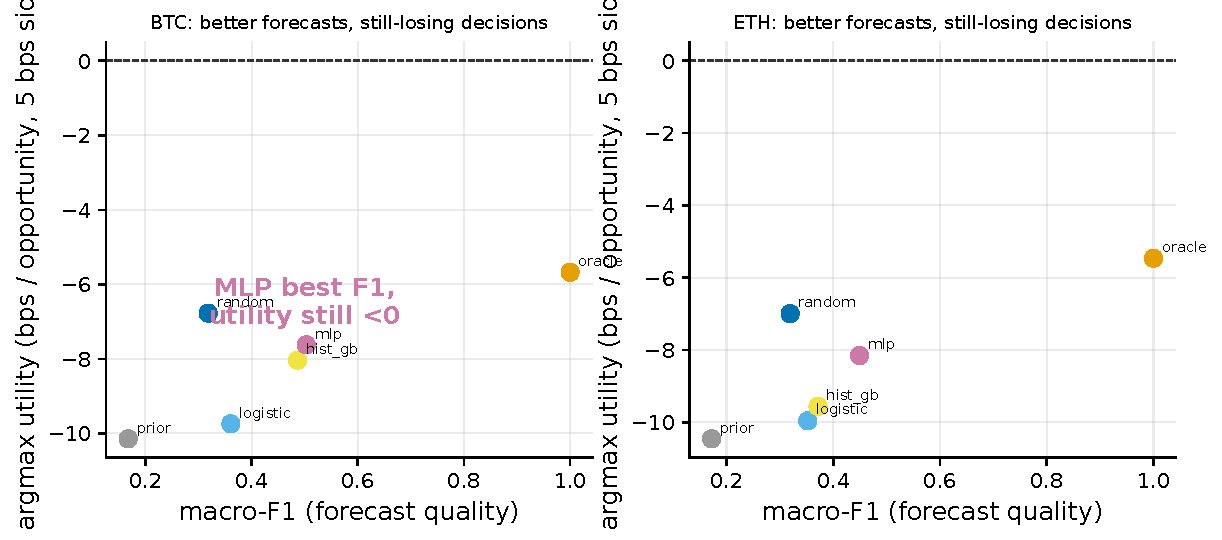
\includegraphics[width=\linewidth]{figures/fig_q17_forecast_decision.pdf}
\caption{\textbf{Q17: better forecasts, still-losing decisions.} Each point is a model
family placed at its macro-F1 (x) and its argmax utility in basis points per opportunity
at $5$ bps per side (y), for BTC (left) and ETH (right). Moving right (better forecasts)
does not move above the dashed zero-utility line: every learned policy trades at a loss,
and the forecast winner (\texttt{mlp}) is not a profitable decision.}
\label{fig:q17}
\end{figure}

\paragraph{The joint gate fails on every contrast.} The pre-registered criterion for
declaring a forecast-to-decision improvement requires both a predictive advantage and a
utility reversal across at least two policy families on six of eight dates. Of the eight
protocol contrasts (one macro-F1 and three utility contrasts per asset), $0$ pass. BTC
shows a significant macro-F1 gain but the confidence and scheduling contrasts fail their
thresholds, and all four ETH contrasts fail. The scheduling policy is negative on four of
eight dates for both assets. A forecast advantage that is real on the score is not a
decision advantage after the policy and cost layer intervene.

\paragraph{Why this is more than a restatement.} That scores and decisions can diverge is
known in principle \citep{falezza2026when, raeth2025forecast, f2017murphy,
timo2023evaluating}, and proper-betting guarantees exist under matched scoring rules and
liquidity conditions \citep{anri2026when}. Our contribution is the matched measurement on
real perpetual-futures data with a frozen joint gate: the divergence is not a corner case
produced by one arbitrary strategy, it is the outcome under the strongest learned
forecaster and three standard policies, and it holds on both assets. The forecasting
leaderboard and the trading leaderboard are different objects, and Q17 shows how far apart
they sit once real costs are paid.
